\section{Method}\label{sec:method}

Fig.~\ref{fig:system} shows the system under test. A question goes to one of seven retrievers, which searches a fixed corpus; the top $k$ passages go to one of two readers; the answer is scored against reference answers. Only the retriever changes between conditions within a reader--dataset cell.

\begin{figure}[t]
\centering
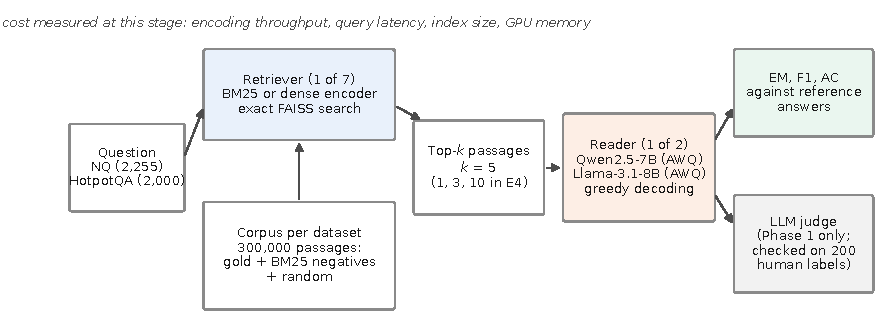
\includegraphics[width=\linewidth]{figs/fig7_system.pdf}
\caption{System under test. Within a reader--dataset cell only the retriever changes. Cost is measured at the retrieval stage. The LLM judge was used only in Phase~1 and was later excluded (Section~\ref{sec:res-judge}).}
\label{fig:system}
\end{figure}

\subsection{Transfer ratio}\label{sec:ratio}
Let $Q$ be a fixed set of generation queries. For retriever $R$ and query $q$, let $h_R(q)\in\{0,1\}$ indicate that at least one gold passage of $q$ is among the top five passages, and let $e_R(q)\in\{0,1\}$ be the exact match of the reader's answer given those five passages. Write $\bar h_R$ and $\bar e_R$ for the means over $Q$. With MiniLM-L6 as the baseline $R_1$, the transfer ratio is
\begin{equation}
T(R) = \frac{\bar e_R - \bar e_{R_1}}{\bar h_R - \bar h_{R_1}}.
\label{eq:ratio}
\end{equation}
Both differences are paired: they use the same queries, the same reader, the same prompt and the same decoding. $T(R)$ is a ratio of mean differences. It is not the probability that one extra hit produces one extra correct answer, because the queries that gain a hit need not be the queries that gain an answer. We report $T(R)$ only if $|\bar h_R-\bar h_{R_1}|$ exceeds 2 percentage points and the Hit@5 difference is significant after Holm correction; otherwise the ratio is marked as not estimable. This rule was fixed in the Phase~1 design to avoid ratios with near-zero denominators.

\paragraph{Decomposition}
Let $a_R=P(e_R=1\mid h_R=1)$ and $b_R=P(e_R=1\mid h_R=0)$ be the EM rates among hits and misses. Then $\bar e_R=\bar h_R a_R+(1-\bar h_R)b_R$, and Eq.~\ref{eq:ratio} splits exactly into
\begin{equation}
T(R) = \underbrace{(a_{R_1}-b_{R_1})}_{\text{baseline hit--miss gap}} + \underbrace{\frac{\bar h_R\,(a_R-a_{R_1}) + (1-\bar h_R)\,(b_R-b_{R_1})}{\bar h_R-\bar h_{R_1}}}_{\text{change in conditional EM}}.
\label{eq:decomp}
\end{equation}
If a better encoder only turned misses into hits and left $a$ and $b$ unchanged, $T(R)$ would equal the baseline gap. The second term shows how far the encoder also changes how useful its hits and misses are. This decomposition was not part of the registered analysis; we report it as a post hoc description.

\subsection{Data}\label{sec:data}
\paragraph{Natural Questions}
We used the BEIR version of Natural Questions \citep{kwiatkowski2019nq,thakur2021beir}: \ev{N.nq.judged} judged test queries and a corpus of 2,681,468 Wikipedia passages. BEIR does not ship short answers, so we joined its queries to NQ-open \citep{lee2019orqa} by normalised question text. The join matched \ev{N.nq.joined} queries; \ev{N.nq.unmatched} had no match and none had more than one. All \ev{N.nq.joined} joined queries form the NQ generation set. Table~\ref{tab:data} in the appendix summarises both datasets and sub-corpora.

\paragraph{HotpotQA}
We used the BEIR version of HotpotQA \citep{yang2018hotpotqa,thakur2021beir}: \ev{N.hp.judged} judged test queries, two gold passages per query, and a corpus of 5,233,329 passages. Answers come from the fullwiki validation release, joined by question id; all queries matched. The generation set is the leading \ev{N.hp.gen} queries of a seeded order (\ev{N.qhp.bridge} bridge and \ev{N.qhp.comparison} comparison questions).

\paragraph{Sub-corpus}
Encoding millions of passages with six encoders exceeds a free GPU budget, so each dataset uses a 300,000-passage sub-corpus. It contains the gold passages of all judged queries, BM25 top-$d$ non-gold passages for every judged query ($d$ = 42 for NQ and 19 for HotpotQA, set by a pre-registered formula), and a seeded random fill. The NQ sub-corpus has \ev{N.sc.nq.gold} gold, \ev{N.sc.nq.bm25} BM25 and \ev{N.sc.nq.rand} random passages; the HotpotQA sub-corpus has \ev{N.sc.hp.gold}, \ev{N.sc.hp.bm25} and \ev{N.sc.hp.rand}. Because every gold passage is present, absolute retrieval scores are higher than on the full corpus. Section~\ref{sec:res-cost} checks whether the ordering of retrievers changes.

\subsection{Retrievers}\label{sec:retrievers}
BM25 used the bm25s library \citep{lu2024bm25s} with the Lucene variant, $k_1=1.2$, $b=0.75$, lower-casing and no stemming or stop-word removal \citep{robertson2009bm25}. The six dense encoders were all-MiniLM-L6-v2 \citep{reimers2019sbert,wang2020minilm}, bge-small, bge-base and bge-large v1.5 \citep{xiao2024cpack}, e5-base-v2 \citep{wang2022e5} and Qwen3-Embedding-0.6B \citep{zhang2025qwen3emb}. Each model ran at a pinned revision in half precision with a maximum of 256 tokens and its documented query and passage prefixes. Dense search used exact inner-product search in FAISS \citep{johnson2021faiss}. Table~\ref{tab:models} in the appendix lists the models, revisions and prefixes.

\subsection{Readers and prompts}\label{sec:readers}
The readers were Qwen2.5-7B-Instruct \citep{qwen2025qwen25} and Llama-3.1-8B-Instruct \citep{grattafiori2024llama3}, both in 4-bit AWQ form \citep{lin2024awq}, served with vLLM \citep{kwon2023vllm} on one T4 each. Decoding was greedy with at most 32 new tokens and a stop at a newline. The main prompt (A1) gives the top $k=5$ passages in rank order, each as ``[i] title / text'', and asks for a short answer (Appendix~\ref{app:prompts}). Two reference conditions bound each cell: closed book (no passages) and gold passages only.

\subsection{Metrics}\label{sec:metrics}
Hit@5 is 1 if at least one gold passage is in the top five. For HotpotQA we also report Both@5, which requires both gold passages. nDCG@10 uses binary gains. EM is 1 if the normalised answer equals a normalised reference answer. Normalisation follows SQuAD (lower case, no punctuation or articles, single spaces) and also removes typographic quotes, en and em dashes and the ellipsis; a plain SQuAD normaliser would change the score of \ev{IC.plain} of \ev{IC.n} answers (\ev{IC.plainpct}). Token F1 and answer containment (AC; a normalised reference occurs in the normalised output) are secondary metrics, because lexical EM undercounts correct answers from language models \citep{kamalloo2023}.

\subsection{Statistical analysis}\label{sec:stats}
All comparisons are paired by query. Binary outcomes use the exact McNemar test \citep{mcnemar1947}. Within each reader--dataset cell, the 21 pairwise retriever comparisons of a metric form one family with Holm correction \citep{holm1979}. Intervals are 95\% percentile bootstrap intervals over queries \citep{efron1993bootstrap} with 10,000 resamples and seed 0; for $T(R)$ the numerator and denominator are resampled together. A secondary model pools the four cells: a logistic generalised estimating equation \citep{liang1986gee} for EM with retriever, dataset and reader as factors, an exchangeable working correlation within query, and empirical (sandwich) standard errors. Agreement between the LLM judge and human labels uses Cohen's $\kappa$ \citep{cohen1960kappa,landis1977}. A non-significant test is reported as ``no difference detected'', not as equivalence.

\subsection{Pre-registered predictions}\label{sec:prereg}
Phase~1 (Qwen reader, NQ) was designed and committed before any data were generated. Before Phase~2 we registered six predictions (Table~\ref{tab:predictions}):
\begin{description}
\item[P1] In each new cell, every reportable $T(R)$ of a dense encoder has an upper 95\% bound below 1.
\item[P2] In each new cell, bge-large and Qwen3-Embedding-0.6B show no Holm-significant EM gain over e5-base-v2.
\item[P3] The nDCG@10 ordering of BM25, MiniLM-L6, bge-small and e5-base-v2 on the sub-corpus holds on the full corpus.
\item[P4] For every retriever, EM at $k=1$ is lower than at $k=5$.
\item[P5] Gold plus four hard negatives gives lower EM than gold plus four random passages.
\item[P6] The position of the gold passage (1, 3 or 5) changes EM.
\end{description}
Fig.~\ref{fig:phases} shows the sessions of both phases. The Qwen--NQ cell and the $k$ ablation for BM25, MiniLM-L6 and bge-large existed before registration. Their P1, P2 and P4 verdicts are therefore not confirmatory, and Table~\ref{tab:predictions} marks them. All other analyses are descriptive or secondary. Appendix~\ref{app:prereg} lists the design documents and their dates.

\begin{figure}[t]
\centering
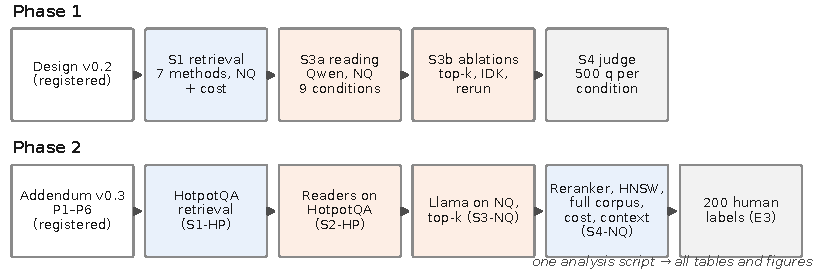
\includegraphics[width=\linewidth]{figs/fig8_phases.pdf}
\caption{Study phases and Kaggle sessions. Each phase started with a dated design document; Phase~2 added the second dataset, the second reader and the additional experiments.}
\label{fig:phases}
\end{figure}

\subsection{Additional experiments}\label{sec:extra}
\paragraph{Top-$k$ (E4)} The Qwen reader answered all NQ queries with $k\in\{1,3,5,10\}$ for all seven retrievers.
\paragraph{Context composition (E12)} On the leading 500 NQ generation queries of the seeded order, the Qwen reader always saw five passages: gold at position 1 plus four hard negatives (M1); gold at position 3 or 5 among the same negatives (M3, M5); gold at position 1 plus four random passages (MR); and the gold passage alone (MG). Hard negatives are the top-ranked BM25 passages that are not labelled gold.
\paragraph{Reranking (E5)} A cross-encoder, bge-reranker-base, reranked the top 50 passages of BM25 and of e5-base-v2 \citep{nogueira2019passage,xiao2024cpack}; the Qwen reader then answered NQ from the reranked top five.
\paragraph{Approximate search (E6)} HNSW indexes \citep{malkov2020hnsw} ($M=32$, efConstruction 200, efSearch 64 and 128) replaced exact search for MiniLM-L6, bge-small and e5-base-v2 on the NQ sub-corpus.
\paragraph{Full corpus (E9)} BM25, MiniLM-L6, bge-small and e5-base-v2 retrieved from the full NQ corpus for all judged queries.
\paragraph{Cost (E7)} For each encoder we measured passage-encoding throughput on 20,000 passages (batch 128, after warm-up, with GPU synchronisation) and batch-1 query-encoding latency on 500 queries, five times in one session.
\paragraph{Judge validation (E3)} In Phase~1, an LLM judge (Mistral-7B-Instruct-v0.3; \citealp{jiang2023mistral}) labelled whether each answer was supported by its passages, for 500 NQ queries per retriever. The author labelled a stratified sample of 200 items without seeing the judge's verdicts. The registered rule was: use the judge if $\kappa\ge0.4$, use it only with a sensitivity analysis if $0.2\le\kappa<0.4$, and exclude it if $\kappa<0.2$.
